% \section{Introduction}

% Recent progress in large-scale multimodal pretraining has produced generalist vision--language--action (VLA) policies~\citep{black2410pi0,bjorck2025gr00t,kim2024openvla,zitkovich2023rt,pertsch2025fast} that integrate perception, language understanding, and control within a unified framework. Trained on large robotic datasets, these models show promising transfer to new tasks, objects, and environments. Despite these capabilities, as illustrated in Fig.~\ref{fig:3rollout}, pretrained VLA policies remain brittle under deployment-time distribution shift. They often struggle to generalize robustly to unseen objects and to reliably follow high-level language instructions, particularly in the presence of distractors. A standard way to improve performance is to finetune the policy on target-task data. However, finetuning is not always desirable or feasible: it requires additional data collection, can overfit to the adaptation distribution, and changes the pretrained policy itself. This raises an important question: \textbf{how can we improve performance on unseen objects and instruction-following accuracy without finetuning the pretrained VLA policy?}



% Test-time steering offers such a training-free alternative. In large language models, steering by sampling multiple candidate outputs and ranking them with a separate judge or scoring model has proven effective for improving reliability without retraining~\citep{kang2025scalable,pi2025mr}. 
% Pretrained VLA policies provide a natural analogue; diffusion-based VLAs~\citep{black2410pi0,bjorck2025gr00t} sample actions through stochastic denoising, while autoregressive VLAs~\citep{kim2024openvla,zitkovich2023rt,pertsch2025fast} sample action sequences from a learned distribution. This stochasticity creates an opportunity to steer the policy by choosing which action chunk to execute.
% The key challenge is that, unlike text outputs, the quality of an action chunk cannot be directly evaluated without executing it in the physical environment. Failed actions can move the robot away from the goal, violate the instruction, or lead to unrecoverable states. Thus, test-time steering for VLAs hinges on a natural question: \textbf{how can we evaluate and compare candidate action chunks before executing them on the robot?}



% \textit{World models}~\citep{agarwal2025cosmos,assran2025v,zhou2411dino} offer a way to bridge this gap by predicting the consequences of actions before execution. Given the current observation and a candidate action chunk, an action-conditioned world model can imagine the future visual state that would result from executing that chunk. These imagined rollouts can then be evaluated by an external, language-conditioned \textit{value model}, enabling look-ahead action evaluation at deployment time. 
% This imagined rollout-and-evaluation mechanism is especially useful in the generalist policy setting because the policy, world model, and value model need not be constrained to the same data distribution. A VLA policy must output executable robot actions and is typically trained on successful robot demonstrations. In contrast, a world model can, in principle, learn from broader interaction data, including successful trajectories, failed attempts, random play, human videos, and cross-embodiment demonstrations. A value model can be broader still, since image-based progress estimation can leverage visual-language pretraining and diverse human or robot data. These components therefore provide complementary capabilities: the policy proposes feasible actions, the world model predicts their consequences, and the value model evaluates whether those consequences align with the instruction.



% \begin{wrapfigure}{r}{0.42\textwidth}
%     \centering
%     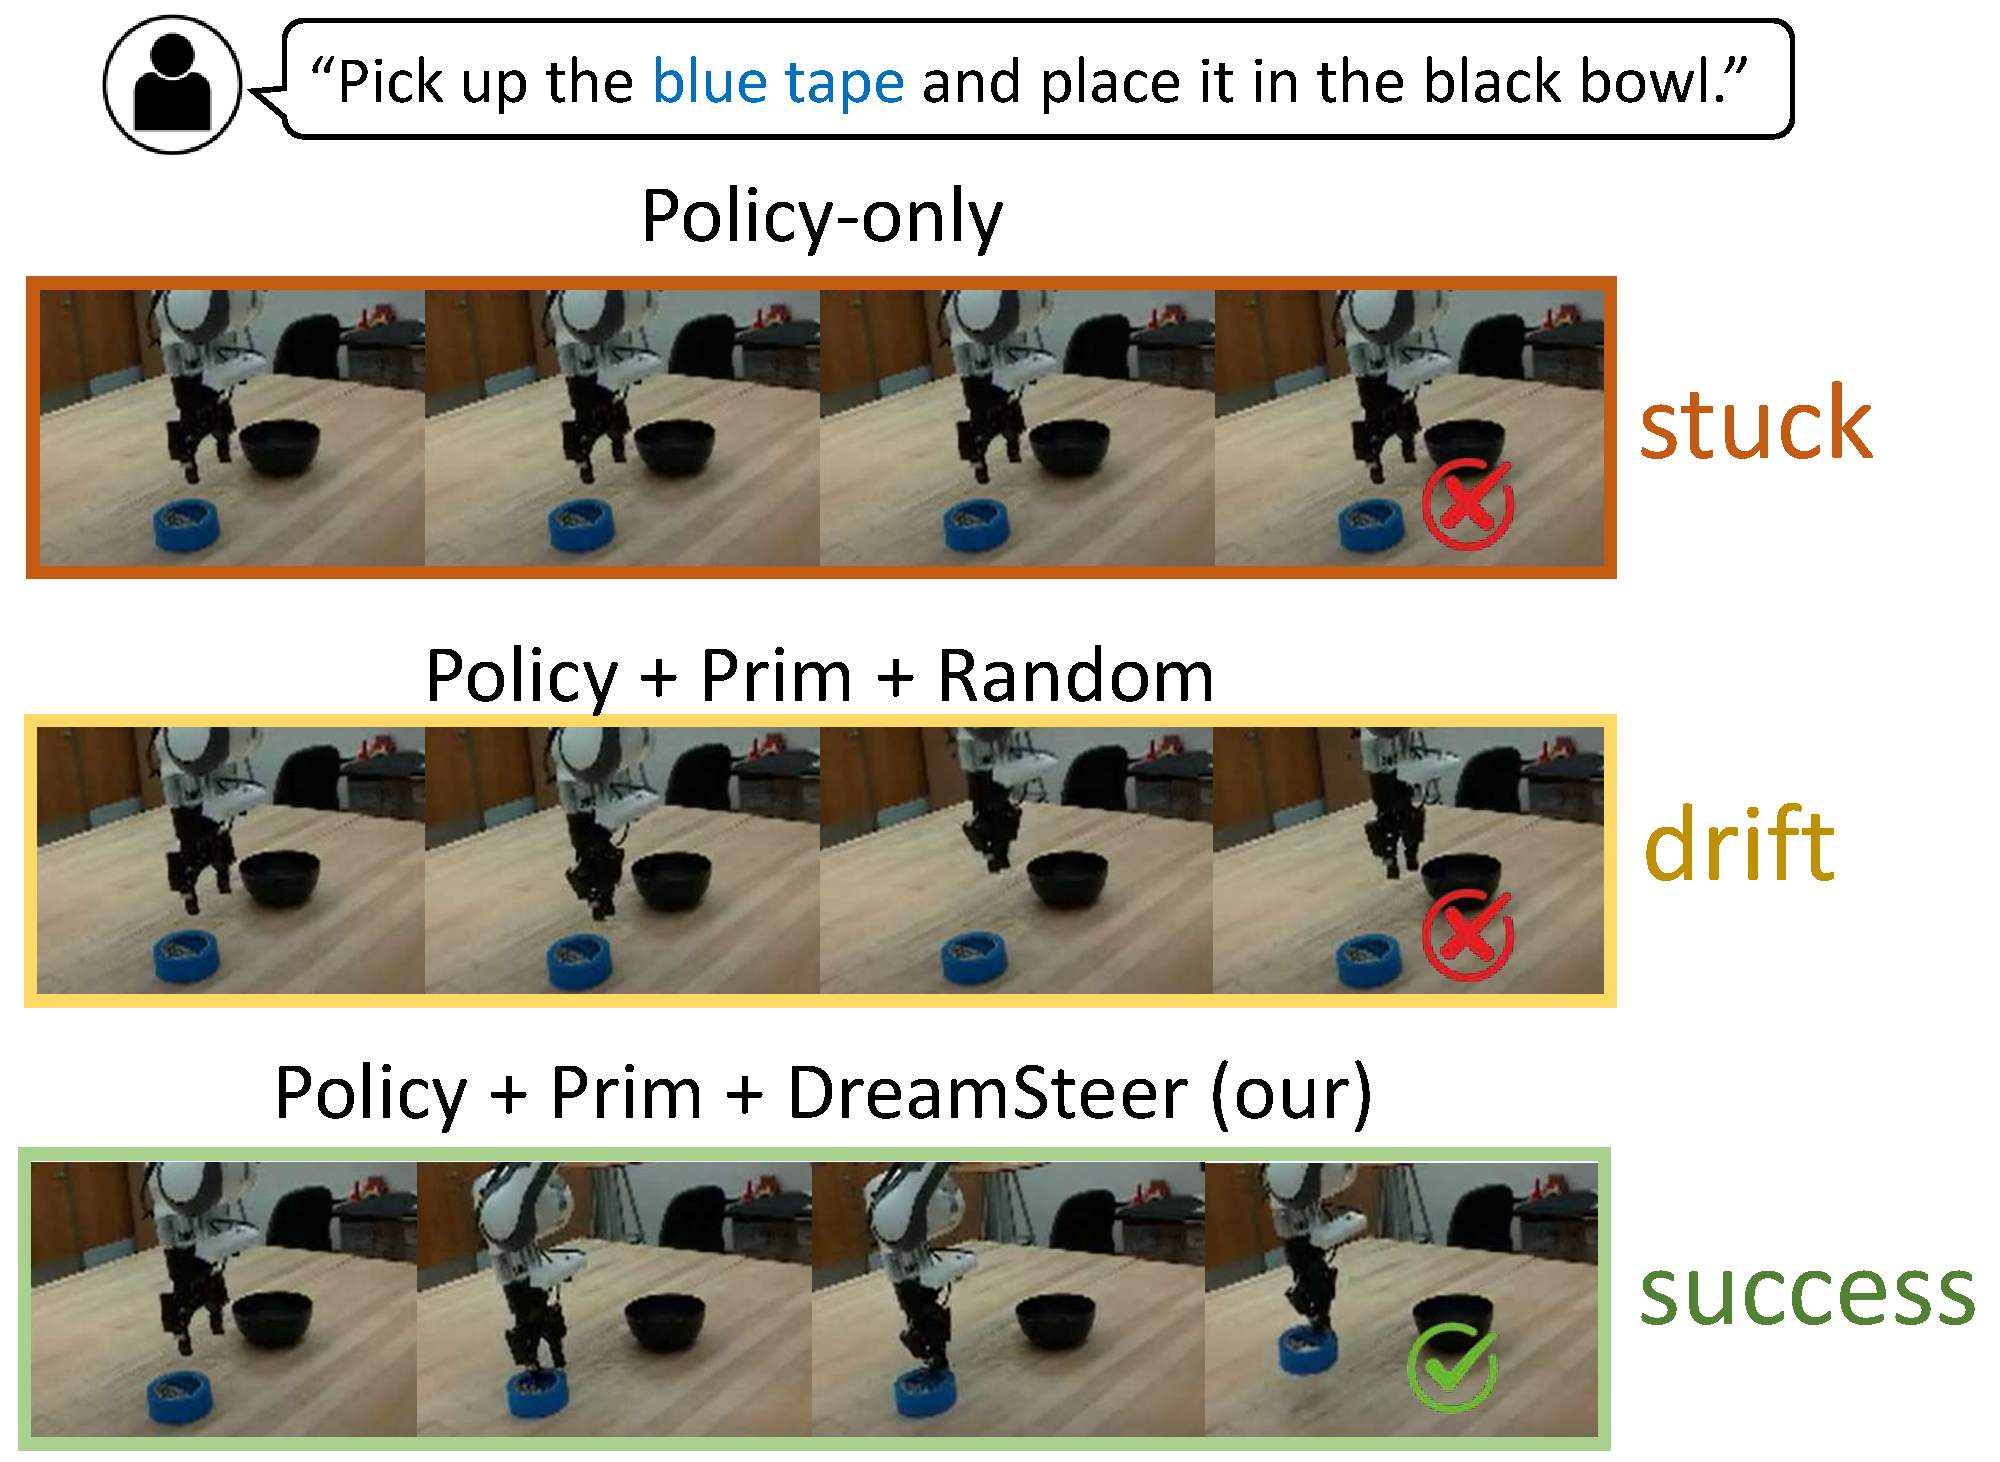
\includegraphics[width=\linewidth]{figures/3rollouts_edited.pdf}
%     \caption{\textbf{\coolname{} improves deployment-time robustness of pretrained policies with zero finetuning.} The base policy becomes stuck, random exploration causes drift, while \coolname{} successfully completes the task.}
%     \label{fig:3rollout}
% \end{wrapfigure}


% In this paper, we present \textbf{\coolname{}}, a deployment-time framework for steering pretrained generalist policies using latent world models with zero finetuning. Our method is shown in Fig.~\ref{fig:dreamsteer}. Given a language instruction and current observation, a pretrained VLA policy first generates multiple candidate action chunks~\citep{zhao2023learning}. We augment these samples with a small set of predefined action primitives to improve candidate coverage. Each candidate is then rolled out with an action-conditioned latent world model, whose predicted latents are decoded into visual observations for evaluation. A language-conditioned value model scores the decoded imagined rollouts, and \coolname{} executes the highest-scoring action chunk in the real environment. Importantly, \coolname{} operates entirely at deployment time: the policy, world model, and value model are kept fixed, and none of them are trained or finetuned on target-environment data.




% Our contributions are summarized as follows:
% \begin{enumerate}
% \item We introduce \textbf{\coolname{}}, a general-purpose test-time steering framework that integrates a pretrained VLA policy, a task-agnostic world model, and a language-conditioned value model, enabling action proposals to be evaluated through imagined rollouts before execution.

% \item Unlike prior approaches that rely on task-specific training or finetuning of one or more components, \coolname{} operates entirely at deployment time by composing pretrained modules, and does not need any finetuning of any of the underlying models. This enables training-free steering of VLA policies under distribution shift.

% \item We evaluate \coolname{} on a real-world robot setup unseen by the underlying modules, including the VLA policy, world model, and value model. \coolname{} improves OOD object manipulation success from 23.75\% to 66.25\%, and improves instruction-following accuracy from 38.75\% to 56.25\% compared to the base $\pi_0$ policy, without finetuning any component on target-environment data.
% \end{enumerate}



%======================tighten version==============================

\section{Introduction}

Recent progress in large-scale multimodal pretraining has enabled VLA policies~\citep{black2410pi0,bjorck2025gr00t,kim2024openvla,zitkovich2023rt,pertsch2025fast} that integrate perception, language understanding, and control within a unified framework. Trained on large-scale robot datasets, these models show promising transfer to new tasks, objects, and environments. However, pretrained VLAs remain brittle under deployment-time distribution shift, often failing on unseen objects or producing behaviors that violate language instructions. While finetuning can improve performance, it requires additional target-domain data and modifies the pretrained policy, which may not be desired or feasible. This raises a key question: \textbf{how can we improve pretrained VLA policies at deployment time without target-domain data finetuning?}

% Test-time steering offers a training-free alternative. 
In the context of large language models, a similar challenge is tackled by \emph{test-time steering} approaches that sample candidate outputs and rerank them using external judges or scoring models to improve reliability without retraining~\citep{kang2025scalable,pi2025mr}. 
Pretrained VLAs provide a natural analogue: diffusion-based policies~\citep{black2410pi0,bjorck2025gr00t} and autoregressive VLAs~\citep{kim2024openvla,zitkovich2023rt,pertsch2025fast} both produce stochastic action samples that can be steered at inference time. However, unlike text outputs, the quality of an action chunk cannot be evaluated directly before execution in the physical world.

World models~\citep{agarwal2025cosmos,assran2025v,zhou2411dino} provide a natural mechanism for evaluating candidate actions before execution. Conceptually, they enable \emph{thinking before acting}. Given the current observation and a candidate action chunk, an action-conditioned world model can predict the resulting future observations. These imagined rollouts can then be ranked by a language-conditioned value model, enabling look-ahead action evaluation at deployment time.

\begin{wrapfigure}{r}{0.47\textwidth}
    \centering
    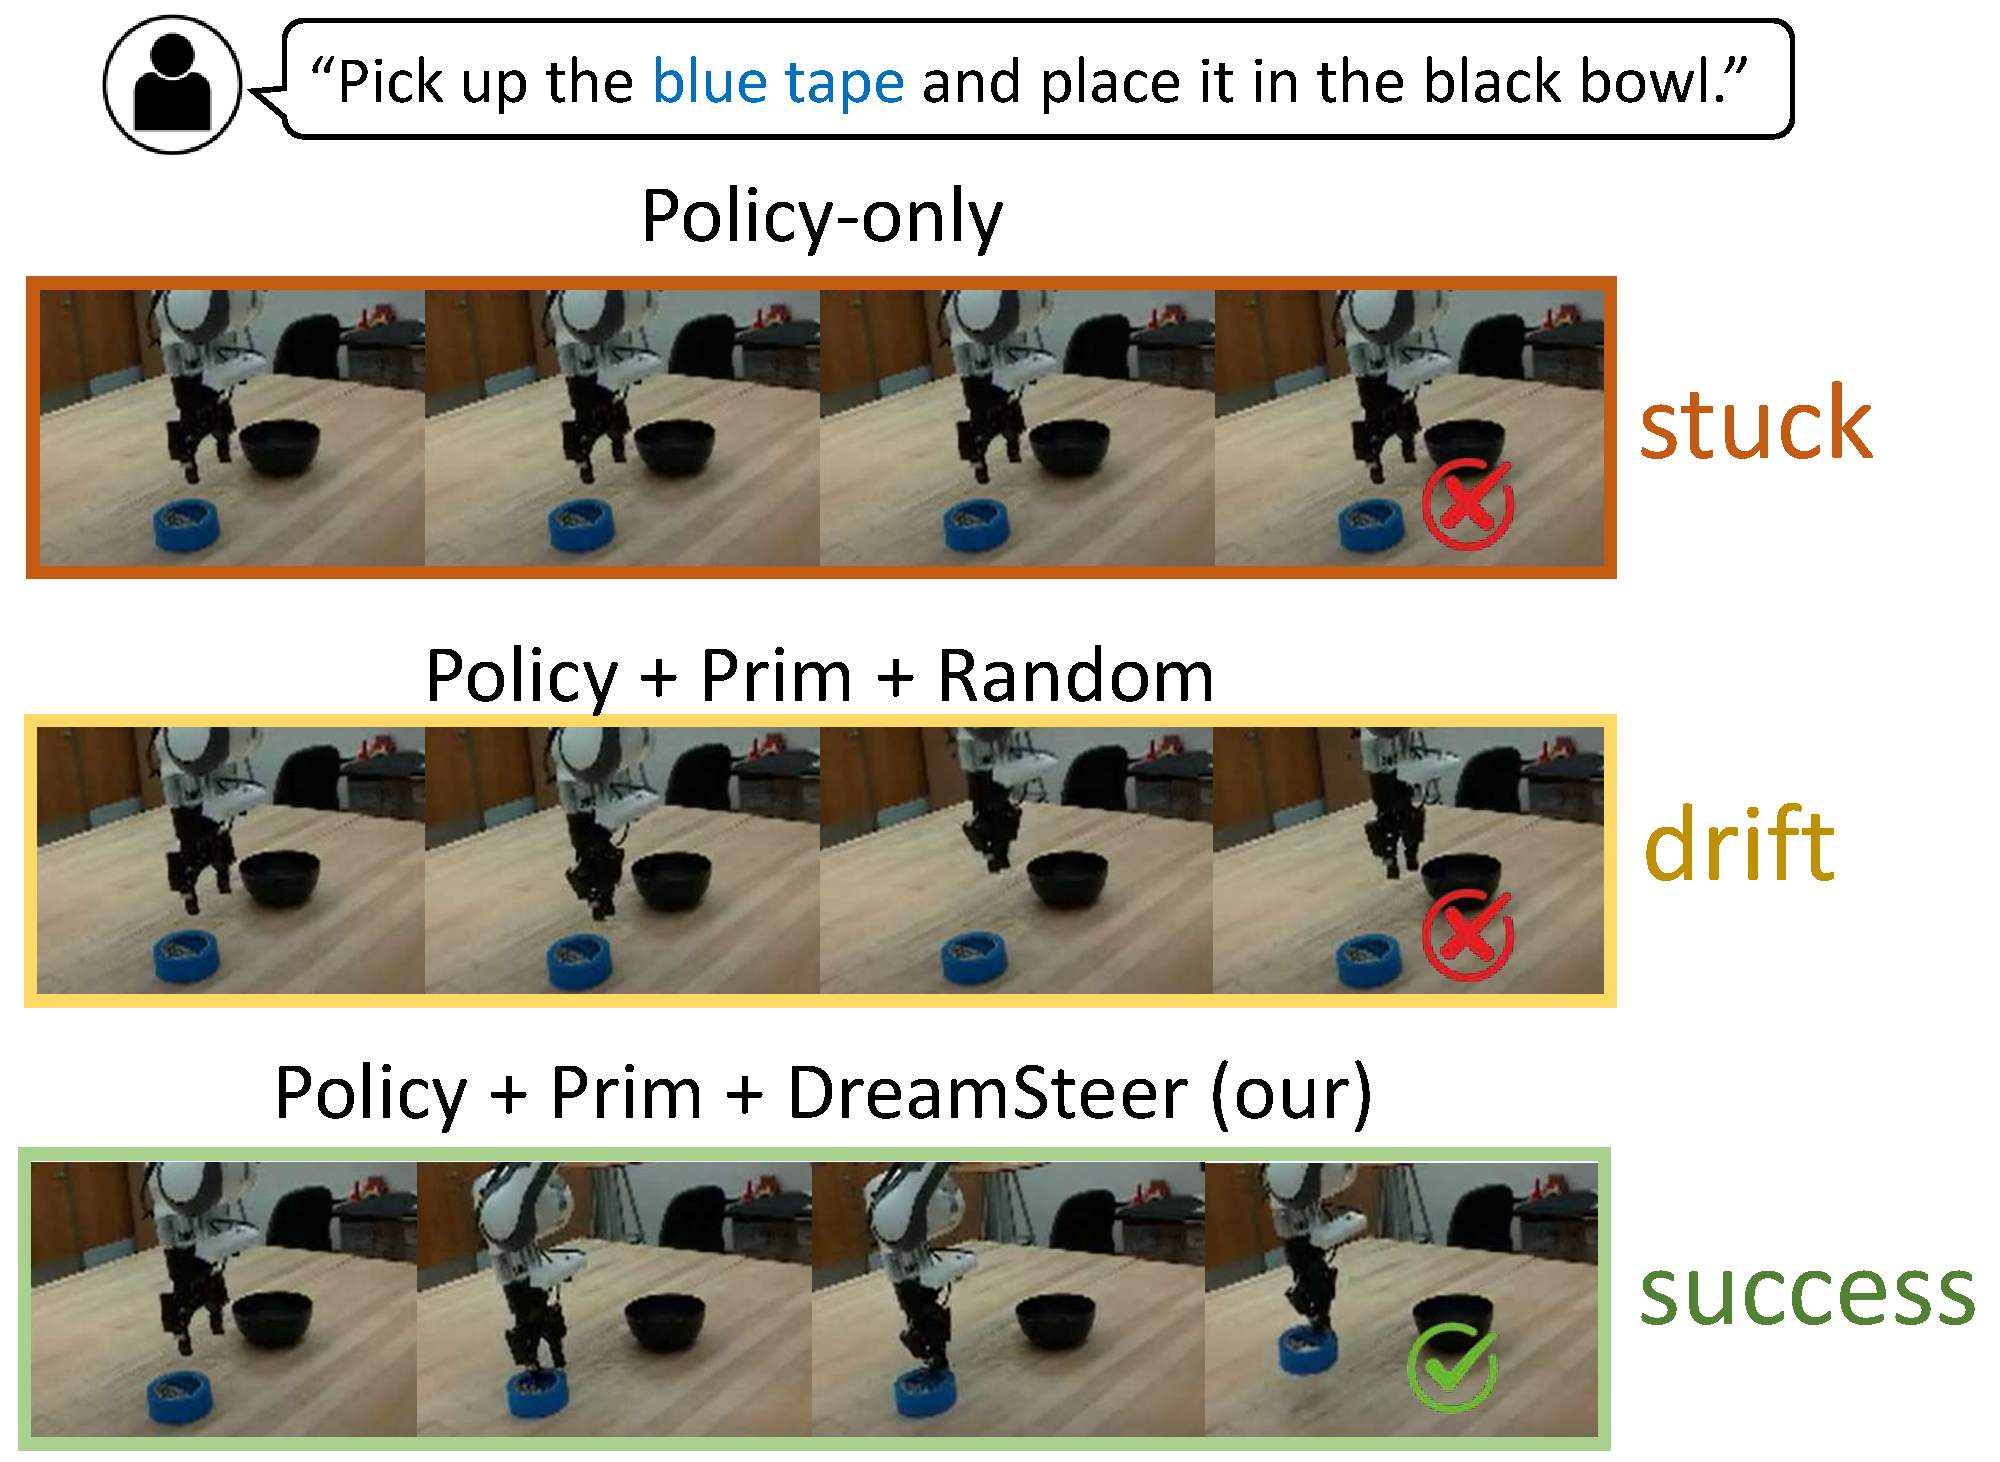
\includegraphics[width=\linewidth]{figures/3rollouts_edited.pdf}
    \caption{\textbf{\coolname{} improves deployment-time robustness} of a pretrained, frozen VLA policy.}
    \label{fig:3rollout}
\end{wrapfigure}

In this paper, we introduce \textbf{\coolname{}}, a deployment-time steering framework for pretrained VLA policies using latent world models with zero finetuning. Given a language instruction and current observation, \coolname{} samples multiple candidate action chunks from a pretrained VLA policy and augments them with predefined motion primitives. An action-conditioned latent world model predicts imagined future observations for each candidate, and a language-conditioned value model ranks the resulting rollouts. \coolname{} then executes the highest-scoring action chunk in the real environment. \textbf{All components remain fixed during deployment, and no target-environment data is used for adaptation}. As illustrated in Fig.~\ref{fig:3rollout}, single-sample policy execution may fail under deployment-time distribution shift, while evaluating multiple imagined futures before execution allows \coolname{} to select more reliable actions.


Our contributions are summarized as follows:
\begin{enumerate}[leftmargin=*, noitemsep, topsep=2pt]
\item We introduce \textbf{\coolname{}}, a deployment-time steering framework that evaluates candidate VLA action chunks through imagined latent-world-model rollouts before execution.

\item \coolname{} composes a pretrained VLA policy, a generalized latent world model, and a language-conditioned value model at deployment time, without finetuning any component on target-environment data.

\item We demonstrate \coolname{} improves OOD object manipulation success from 23.75\% to 66.25\%, and instruction-following accuracy from 38.75\% to 56.25\% over the $\pi_0$ VLA policy.
\end{enumerate}